\documentclass{article}
\usepackage{graphicx}

\begin{document}

\title{Introduction to \LaTeX{}}
\author{Author's Name}

\maketitle

\begin{abstract}
	Hello there
	Hello there
	Hello there
	Hello there
	Hello there
	Hello there
	Hello there
	Hello there
	Hello there
\end{abstract}

\section{Introduction}
Here is the text of your introduction. Indeed!

\begin{equation}
	\frac{5 + x}{y} = 29
\end{equation}

\begin{equation}
    \label{simple_equation}
    \alpha = \sqrt{ \beta }
\end{equation}

\subsection{Subsection Heading Here}
Write your subsection text here. Text Text Text.

\begin{figure}
    \centering
    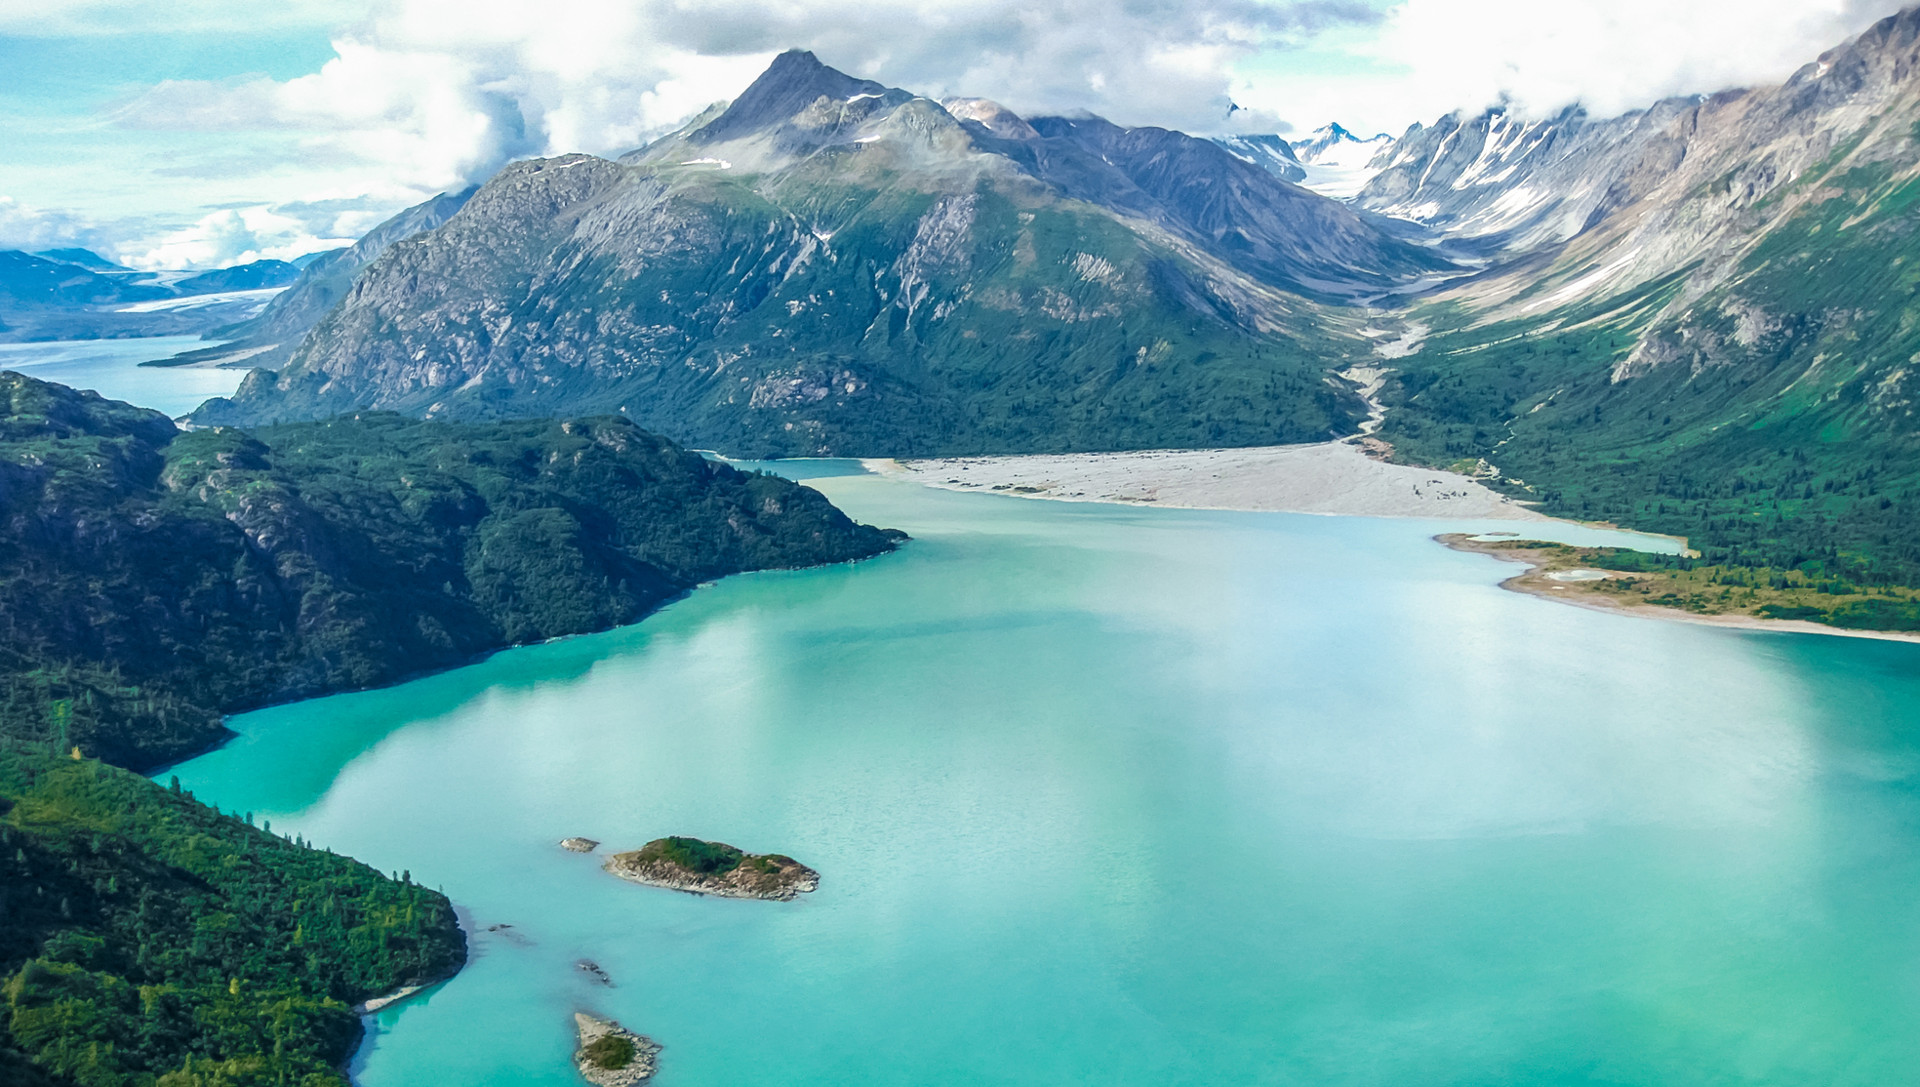
\includegraphics[width=3.0in]{myfigure}
    \caption{Simulation Results}
    \label{simulationfigure}
\end{figure}

\section{Conclusion}
Write your conclusion here.

\end{document}

